\documentclass{article}
%% \usepackage{times}
\usepackage{latexsym}
\usepackage{url}
\usepackage{hyperref}
\usepackage{listings}
\usepackage{graphicx}
\graphicspath{ {C:\Users\ADMIN\Desktop\Cazuri de test} }
\hypersetup{colorlinks=true}
\usepackage{enumitem,amssymb}
\newlist{todolist}{itemize}{4}
\setlist[todolist]{label=$\square$}


\begin{document}
\pagenumbering{arabic}
% top matter
\title{\huge{Calea minim\u{a} dintre dou\u{a} v\^{a}rfuri la grafuri orientate}}
\date{\Large{\today}}
\maketitle
\begin{center}
\vspace{30 mm}

\begin{tabbing}
\indent{\huge{Student:}} {\huge{Anghel Florina-C\u{a}t\u{a}lina} }\\
\\\vspace{10 mm}
\indent{\huge{Grupa:}} {\huge{CR1.1} }\\
\\\vspace{10 mm}
\indent{\huge{Specializarea:}} {\huge{Calculatoare cu predare \^{i}n limba rom\^{a}n\u{a}}}\\
\\\vspace{10 mm}


\indent{\huge{Anul \^{i}nt\^{a}i}}
\end{tabbing}
\end{center}
\clearpage

% sections

\section{Introducere}
\subsection{Enun\c{t}ul problemei}
Implementa\c{t}i doi algoritmi care s\u{a} determine calea minim\u{a} dintre dou\u{a} v\^{a}rfuri dintr-un graf orientat. 
\\Pentru a rezolva aceast\u{a} problem\u{a}, am ales s\u{a} implementez:
\begin{itemize}
    \item Algoritmul lui Dijkstra
    \item Algoritmul Floyd-Warshall
\end{itemize}

\subsection{Func\c{t}ii folosite}
Este un proiect modular, care contine 3 fi\c{s}iere cu extensia .c si dou\u{a} fi\c{s}iere de tip header. 

\^{I}n matrix.c am implementat:
\begin{itemize}
    \item O func\c{t}ie care s\u{a} genereze \^{i}n mod aleator numarul de v\^{a}rfuri ale grafului
    \item O func\c{t}ie pentru generarea unui numar aleator pe care o folosesc la generarea v\^{a}rfului start, dar \c{s}i a v\u{a}rfului destina\c{t}ie
    \item O func\c{t}ie pentru generarea matricei de adiacen\c{t}\u{a}
    \item O func\c{t}ie pentru generarea matricei de cost pe baza celei de adiacen\c{t}\u{a}
    \item Dou\u{a} func\c{t}ii pentru afi\c{s}area matricelor
\end{itemize}

In shortest\_length\_path.c am implementat:
\begin{itemize}
    \item Func\c{t}ia Dijkstra, de tip void
    \item Func\c{t}ia Floyd-Warshall, de tip void
    \item O func\c{t}ie push\_beginning, pe care am folosit-o pentru a afi\c{s}a calea \^{i}n cazul algoritmului Floyd-Warshall, apel\^{a}nd-o pentru o stiv\u{a}
    \item O func\c{t}ie pop\_beginning\_list pentru a extrage elementele din stiv\u{a}
\end{itemize}

In main.c se afl\u{a} func\c{t}ia main.

Fi\c{s}ierele de tip header sunt matrix.h \c{s}i shortest\_length\_path.h



\section{Algoritmi folosi\c{t}i}

\begin{itemize}
    \item Algoritmul lui Dijkstra\\
    La acest algoritm, se memoreaz\u{a} elementele din matricea de cost \^{i}ntr-un vector denumit  distance \c{s}i se ini\c{t}ializeaz\u{a} elementele vectorului visited cu 0, acest vector ilustr\^{a}nd dac\u{a} v\^{a}rful respectiv a fost sau nu parcurs. Acest algoritm determin\u{a} calea minim\u{a} pentru toate v\^{a}rfurile, dar a fost particularizat pentru a afi\c{s}a doar calea minim\u{a} \c{s}i distan\c{t}a de la un v\^{a}rf start p\^{a}n\u{a} la unul destina\c{t}ie. Variabila local\u{a} count este folosit\u{a} pentru a nu dep\u{a}\c{s}i num\u{a}rul de v\^{a}rfuri ale grafului. \\
    C\^{a}t timp nu este dep\u{a}\c{s}it num\u{a}rul de v\^{a}rfuri, se calculeaz\u{a} distan\c{t}a minim\u{a} \c{s}i se re\c{t}ine valoarea iteratorului \^{i}n variabila next\_node. Se testeaz\u{a} dac\u{a} exist\u{a} o cale mai eficient\u{a} \^{i}ntre v\^{a}rfuri. Se testeaz\u{a} dac\u{a} exist\u{a} o alt\u{a} cale mai eficient\u{a} \c{s}i dac\u{a} r\u{a}spunsul este afirmativ, atunci se actualizeaz\u{a} vectorul distan\c{t}\u{a} \c{s}i vectorul predecessor re\c{t}ine nextnode.Variabila count se incrementeaz\u{a} pentru a arata c\u{a} a mai fost parcurs un v\^{a}rf. Apoi se afiseaz\u{a} distan\c{t}a \c{s}i calea minim\u{a} dintre cele dou\u{a} v\^{a}rfuri.
    \begin{lstlisting}
    Dijkstra(adj,cost,n,start,dest)
    1.    for i = 0, n - 1 execute
    2.        distance[i] <- cost[start][i]
    3.        predecessor[i] <- start
    4.        visited[i] <- 0
    5.    distance[start] <- 0
    6.    visited[start] <- 1
    7.    count <- 1
    8.    while count < n - 1 execute
    9.        min_dist <- inf
    10.        for i = 0, n - 1 execute
    11.            if distance[i] < min_dist and !visited[i] then
    12.                min_dist <- distance[i]
    13.                next_node <- i
    14.        visited[next_node] <- 1
    15.        for i = 0, n - 1 execute
    16.          if !visited[i] then
    17.            if min_dist + cost[next_node][i] < distance[i] then
    18.                distance[i] <- min_dist + cost[next_node][[i]
    19.                predecessor[i] <- next_node
    20.    count <- count + 1
    21.    for i = 0, n - 1 execute
    22.         if i != start then
    23.             if i = dest then
    24.                write distance[i]
    25.                write i
    26.                j <- i
    27.                repeat
    28.                    j <- predecessor[j]
    29.                    write j
    30.                while j != start
    \end{lstlisting}
    \item Algoritmul Floyd-Warshall\\
    La acest algoritm, se ini\c{t}ializeaz\u{a} matricea distan\c{t}elor cu elementele matricei de cost. Apoi se adaug\u{a} toate v\^{a}rfurile ca v\^{a}rfuri intermediare, se iau toate v\^{a}rfurile ca v\^{a}rfuri surs\u{a} \c{s}i apoi, se iau toate v\^{a}rfurile ca v\^{a}rfuri destina\c{t}ie. La fel ca \c{s}i Dijkstra, algoritmul Floyd-Warshall determin\u{a} distan\c{t}a minim\u{a} pentru toete perechile de v\^{a}rfuri din graf.\\
    \^{I}n cazul \^{i}n care costul parcurgerii printr-un v\^{a}rf intermediar e mai mic dec\^{a}t cel al parcurgerii directe, atunci la distan\c{t}a de la acel moment de timp se adaug\u{a} distan\c{t}a parcurs\u{a} prin nodul intermediar \c{s}i se re\c{t}ine acest varf, altfel se parcurge calea direct\u{a} \c{s}i se re\c{t}ine v\^{a}rful parcurs. Apoi urmeaz\u{a} afi\c{s}area distan\c{t}ei minime \c{s}i a c\u{a}ii minime.\\
    La acest algoritm, pentru a afi\c{s}a calea minim\u{a} am construit o stiv\u{a} \^{i}n care s\u{a} se re\c{t}in\u{a} v\^{a}rfurile intermediare. Prima dat\u{a} se va afi\c{s}a primul v\^{a}rf \c{s}i se va testa dac\u{a} path[iterator\_1][destination\_node] este diferit de -1, caz \^{i}n care se afi\c{s}eaz\u{a} v\^{a}rful destina\c{t}ie, -1 \^{i}nsemn\^{a}nd c\u{a} nu exist\u{a} noduri intermediare. 
    \begin{lstlisting}
    Floyd-Warshall(cost_matrix, n, start, destination)
    1. build the stack
    2. for i = 0, n-1 execute
    3.     for j = 0, n-1 execute
    4.          path[i][j] <- -1
    5.          dist[i][j] <- cost_matrix[i][j]
    6. var <- 0
    7. for i = 0, n-1 execute
    8.      if dist[start][i] != inf
    9.          var <- 1
    10.if var = 0 then
    11.     write "The start vertex has no connection"
    12.     exit
    13.for k = 0, n-1 execute
    14.     for i = 0, n-1 execute
    15.         for j = 0, n-1 execute
    16.             for l = 0, n-1 execute
    17.                 if dist[i][j] > dist[i][k]+dist[k][j] then
    18.                     dist[i][j] <- dist[i][k]+ dist[k][j]
    19.                     path[i][j] <- k
    20.i <- start
    21.j <- destination
    22.write start
    23.while i != destination and path[i][destination] != -1 execute
    24.     push_begining(head_stack, path[i][destination])
    25.     j <- path[i][destination]
    26.     aux <- j
    27.     while path[i][j] != -1
    28.         push_begining(head_stack, path[i][j])
    29.         j <- path[i][j]
    30.     if path[i][j] = -1 then
    31.         i <- aux
    32.         while head_stack->next != NULL execute
    33.             write pop_begining_list(head_stack)
    34.         j <- destination
    35. write destination
    36. write "Do you want to print the path matrix?"
    37. write "Answer with Yes or No"
    38. read answer
    39. if strcmp(answer, "Yes") = 0 then
    40.     for i = 0, n-1 execute
    41.        for j = 0, n-1 execute
    42.             write path[i][j]
    \end{lstlisting}
\end{itemize}
\section{Date experimentale (Generarea matricelor \c{s}i a v\^{a}rfurilor)}
Pentru a genera num\u{a}rul de noduri, am folosit func\c{t}ia rand()\%, apel\^{a}nd-o la \^{i}nceput prin srand((unsigned) (&t)). \^{I}n func\c{t}ia main, pentru a acoperi cazurile \^{i}n care num\u{a}rul de v\^{a}rfuri generat aleator este 0 sau 1, am introdus anumite condi\c{t}ii, care determin\u{a} ie\c{s}irea din program. Din cauza faptului c\u{a} de cele mai multe ori v\^{a}rful surs\u{a} \c{s}i v\^{a}rful destina\c{t}ie generate \^{i}n mod aleator coincideau, am introdus o etichet\u{a} care \^{i}mi permite reluarea gener\u{a}rii v\^{a}rfului destina\c{t}ie \c{s}i modificarea acestuia astfel \^{i}ncat el s\u{a} fie diferit de cel surs\u{a} \c{s}i s\u{a} nu depa\c{s}easc\u{a} num\u{a}rul de v\^{a}rfuri.\\
Pentru utilizarea eficient\u{a} a memoriei, matricele au fost alocate dinamic si initializate cu 0 prin utilizarea func\c{t}iei calloc pentru a scurta timpul de execu\c{t}ie. Tot cu acest scop, dar \c{s}i datorit\u{a} corectitudinii teoretice, indicii matricelor \c{s}i num\u{a}ratoarea v\^{a}rfurilor \^{i}ncep de la zero.\\
Matricea de adiacen\c{t}\u{a} are pe diagonala principal\u{a} zero, ea nu este simetric\u{a} fa\c{t}\u{a} de diagonala principal\u{a} deoarece se trateaz\u{a} cazul \^{i}n care graful este orientat. Dac\u{a} elementul de deasupra diagonalei principale este 1, atunci cel de pe pozi\c{t}ia simetric\u{a} \^{i}n func\c{t}ie de diagonala principal\u{a} va avea valoarea zero deoarece se dore\c{s}te eliminarea intr\u{a}rii \^{i}ntr-o bucla infinit\u{a}. \^{I}ns\u{a} dac\u{a} elementul de deasupra diagonalei principale este zero, atunci pentru elementul de pe pozi\c{t}ia simetric\u{a} lui se va genera aleator. Matricea de cost este generat\u{a} pe baza matricei de adiacen\c{t}\u{a}, av\^{a}nd pe diagonala principal\u{a} zero, iar acolo unde \^{i}n matricea de adiacen\c{t}\u{a} este unu, se genereaz\u{a} aleator un num\u{a}r. \^{I}n cazul \^{i}n care \^{i}n matricea de adiacen\c{t}\u{a} elementul are valoarea zero \c{s}i nu se afl\u{a} pe diagonala principal\u{a}, atunci \^{i}n matricea de cost se pune infinit, pentru c\u{a} nu s-a calculat \^{i}nc\u{a} distan\c{t}a p\^{a}n\u{a} la acel v\^{a}rf prin v\^{a}rfuri intermediare.

\section{Complexitatea algoritmilor}
Pentru a eviden\c{t}ia eficien\c{t}a algoritmilor, am ales doi algoritmi care au complexit\u{a}ti diferite. Primul algoritm, algoritmul lui Dijkstra este foarte eficient din punctul de vedere al timpului necesar execu\c{t}iei sale.\\
Pentru algoritmul Dijkstra, timpul de execu\c{t}ie este egal cu $O(|E| + |V|^2)$, adic\u{a} $O(|V|^2)$, unde E este num\u{a}rul de muchii \c{s}i V este num\u{a}rul de v\^{a}rfuri. Timpul este acesta pentru c\u{a} este timpul maxim al unor bucle combinate, \^{i}n acest caz, fiind vorba de o bucl\u{a} for \c{s}i una while. Deci timpul de execu\c{t}ie devine $O(|V|^2)$.\\
La algoritmul Floyd-Warshall, timpul de execu\c{t}ie este dat de cele patru bucle for combinate, deci timpul este $\Theta(V^4)$.\\
L\u{a}s\^{a}nd la o parte ace\c{s}ti algoritmi, o alt\u{a} secven\u{a} care poate \^{i}ncetini programul este cea de regenerare a v\^{a}rfului destina\c{t}ie deoarece se verific\u{a} dac\u{a} este diferit de cel start \c{s}i dac\u{a} se afl\u{a} \^{i}n intervalul [0, V - 1], unde V este num\u{a}rul de v\^{a}rfuri.


\section{Rezultate \c{s}i concluzii}
Dup\u{a} mai multe teste, am constatat c\u{a} \^{i}n pu\c{t}ine cazuri, cei doi algoritmi afi\c{s}eaz\u{a} c\u{a}i diferite deoarece exist\u{a} mai multe c\u{a}i care au acela\c{s}i cost \c{s}i leag\u{a} acelea\c{s}i v\^{a}rfuri. \^{I}ns\u{a} exist\u{a} c\^{a}teva teste negative, adic\u{a} teste \^{i}n care cele dou\u{a} c\u{a}i afi\c{s}ate difer\u{a}, problema fiind la cel de-al doilea algoritm pentru c\u{a} exclude v\^{a}rfuri (de exemplu, figura a patra ilustreaz\u{a} un astfel de test). Dup\u{a} mai multe teste, am constatat c\u{a} timpul de execu\c{t}ie este de c\^{a}teva secunde, dar se poate extinde \c{s}i la c\^{a}teva minute deoarece, atunci c\^{a}nd se genereaz\u{a} v\^{a}rful destina\c{t}ie, este testat dac\u{a} este diferit de cel de start \c{s}i dac\u{a} se afl\u{a} \^{i}n intervalul de defini\c{t}ie \c{s}i existen\c{t}\u{a} al v\^{a}rfurilor, \^{i}n caz contrar, fiind regenerat.\\
\^{I}n fig. 1, este prezentat un caz de test pozitiv, adic\u{a} un caz \^{i}n care rezultatele de la cei doi algoritmi coincid.\\
\begin{figure}[htp]
\centering
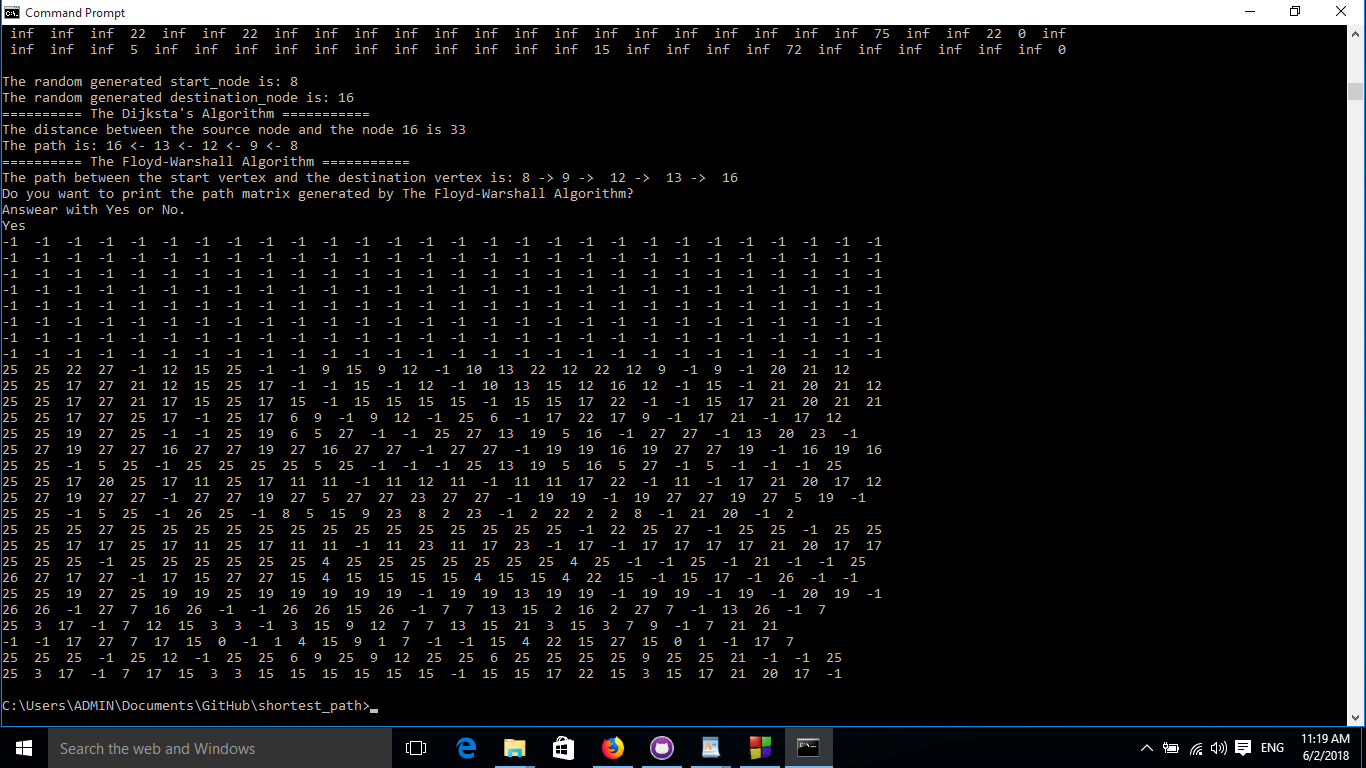
\includegraphics[width=12cm]{Test.png}
\caption{Acesta este un caz de test.}
\label{fig:1}
\end{figure}
\\
\^{I}n figura a doua, este un caz de test \^{i}n care cele dou\u{a} c\u{a}i nu coincid, dar acest test este pozitiv deoarece calea nu este unic\u{a}, adic\u{a} pot exista mai multe c\u{a}i diferite care s\u{a} uneasc\u{a} dou\u{a} v\^{a}rfuri \c{s}i s\u{a} aib\u{a} acela\c{s}i cost.\\
\begin{figure}[htp]
\centering
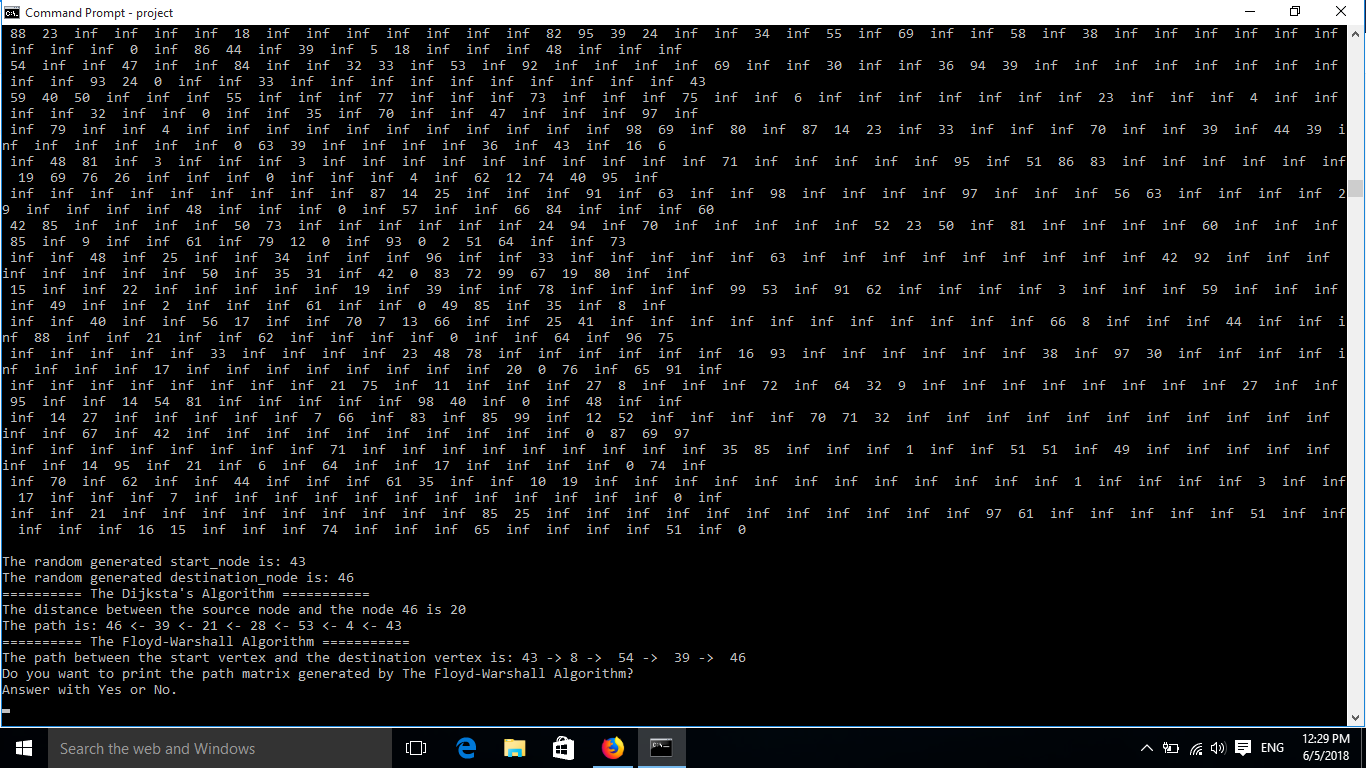
\includegraphics[width=12cm]{Test2.png}
\caption{Acesta este un alt caz de test.}
\label{fig:2}
\end{figure}



\^{I}n figura 3 este prezentat un alt caz pozitiv.\\
\begin{figure}[htp]
\centering
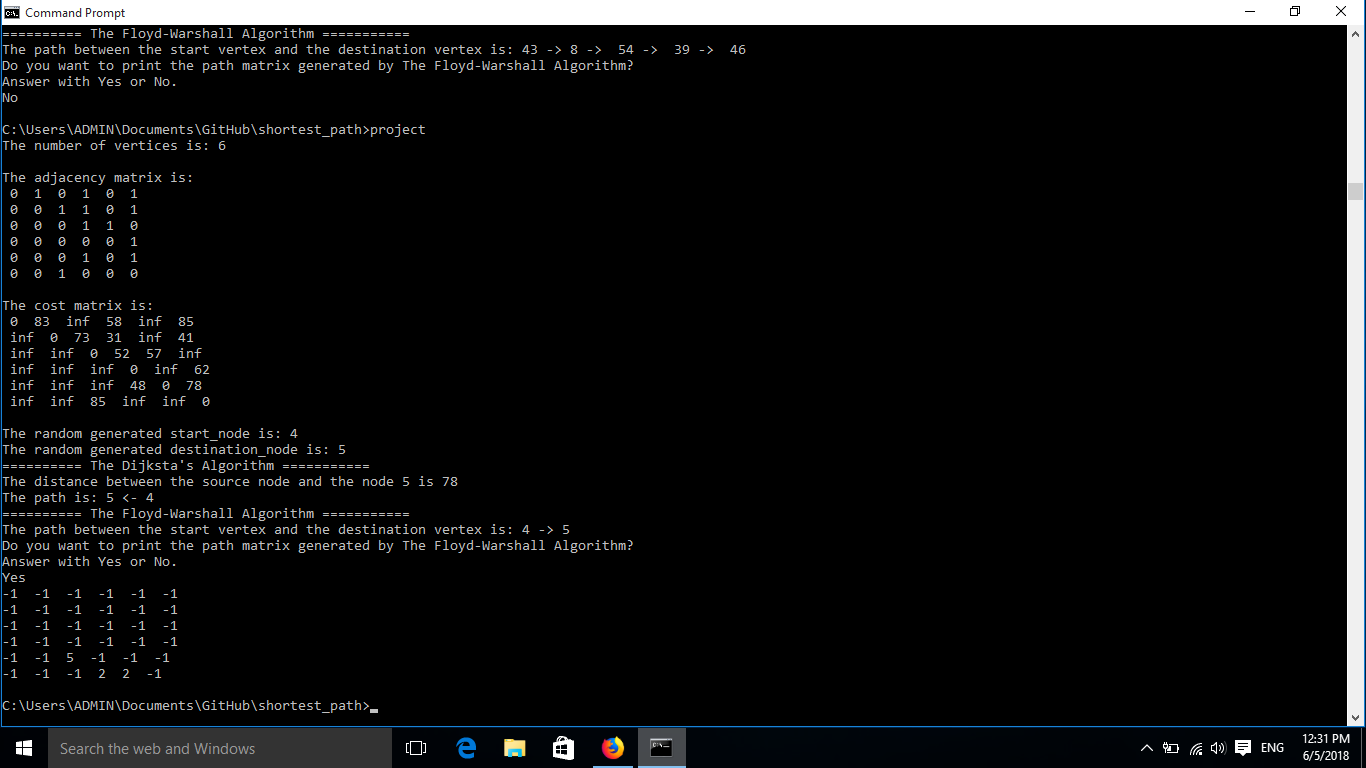
\includegraphics[width=12cm]{Test1.png}
\caption{Acesta este un alt caz de test.}
\label{fig:3}
\end{figure}



\^{I}n figura 4 este prezentat un caz de test negativ, \^{i}n care cei doi algoritmi dau c\u{a}i diferite. Mai exact, \^{i}n aceast\u{a} situa\c{t}ie, algoritmul Floyd-Warshall afi\c{s}eaz\u{a} cu un v\^{a}rf intermediar \^{i}n minus.
\begin{figure}[htp]
\centering
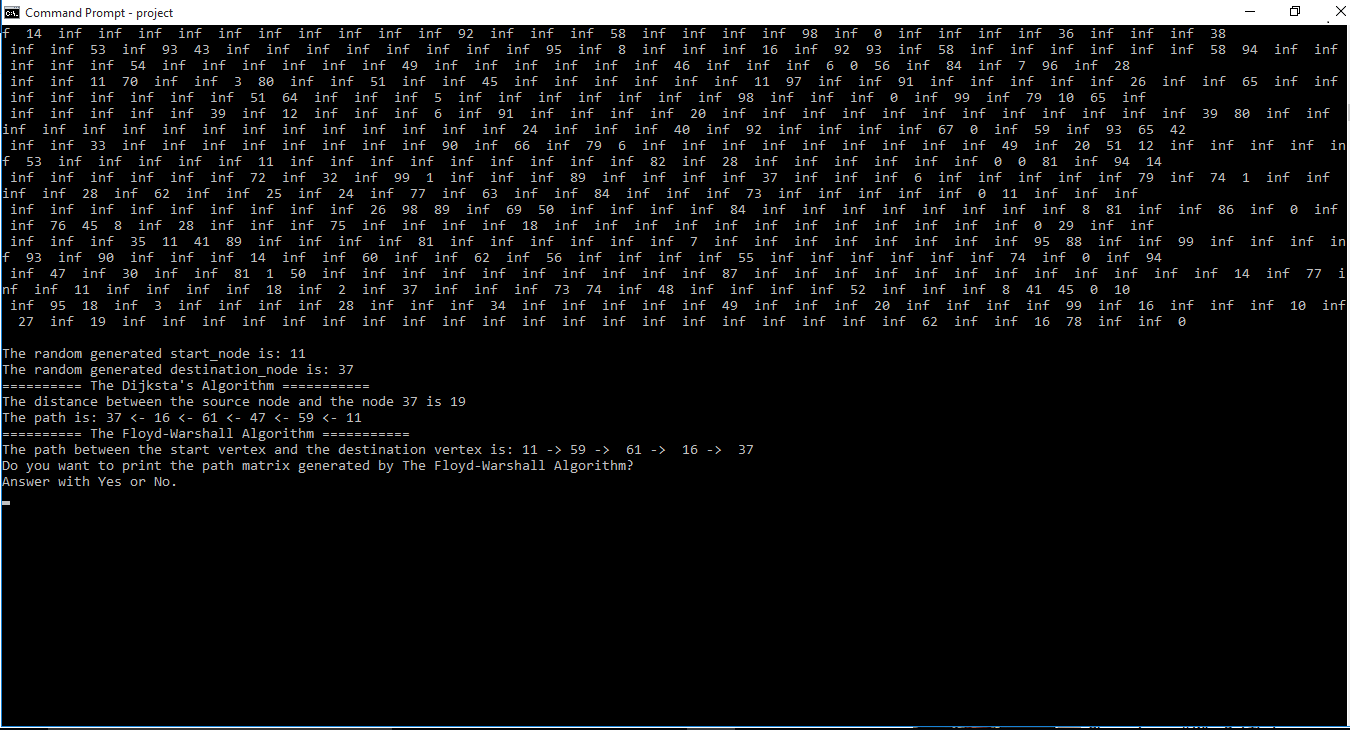
\includegraphics[width=12cm]{Test3.png}
\caption{Acesta este un caz de test negativ.}
\label{fig:4}
\end{figure}\\

\clearpage
\^{I}n concluzie, \^{i}n urma realiz\u{a}rii acestui proiect, mi-am \^{i}mbog\u{a}\c{t}it cuno\c{s}tin\c{t}ele legate de proiectarea algoritmilor, de compilarea \^{i}n linie de comand\u{a}, de utilizarea unui Makefile \c{s}i am exersat lucrul cu aplica\c{t}iile Github, Doxygen \c{s}i ShareLaTeX.
\section{Referin\c{t}e}
\begin{itemize}
\item Wikipedia: https://en.wikipedia.org/wiki/Dijkstra\%27s\_algorithm
\item https://www.geeksforgeeks.org/greedy-algorithms-set-6-dijkstras-shortest-path-algorithm/
\item https://www.geeksforgeeks.org/dynamic-programming-set-16-floyd-warshall-algorithm/
\item Wikipedia: https://en.wikipedia.org/wiki/Floyd\%E2\%80\%93Warshall\_algorithm

\end{itemize}
\end{document}
